\chapter{Aplicação de Monitoramento}
\label{chap4}

{\color{red}
Após o detalhamento da arquitetura e dos componentes do sistema de monitoramento, este capítulo apresenta as aplicações práticas da solução desenvolvida. São abordados os dois mecanismos principais responsáveis pela visualização e notificação das métricas coletadas: os \foreign{dashboards} e os sistemas de alertas.

Na primeira seção, é detalhado o dashboard implementado, incluindo os gráficos e visualizações criados, os códigos PromQL utilizados nas consultas correspondentes e os procedimentos de processamento dos dados. A segunda seção descreve o sistema de alertas, abrangendo as regras de disparo de notificações, a configuração dos pontos e canais de contato, bem como a experiência prática obtida com os diferentes sistemas de alertas disponíveis no ecossistema adotado. A terceira seção apresenta um caso de uso prático, ilustrando a aplicação do sistema de monitoramento em um cenário real.

\section{Dashboards}
\label{section:Dashboards}

\begin{figure}[h]
\centering
\setlength{\abovecaptionskip}{-20pt}
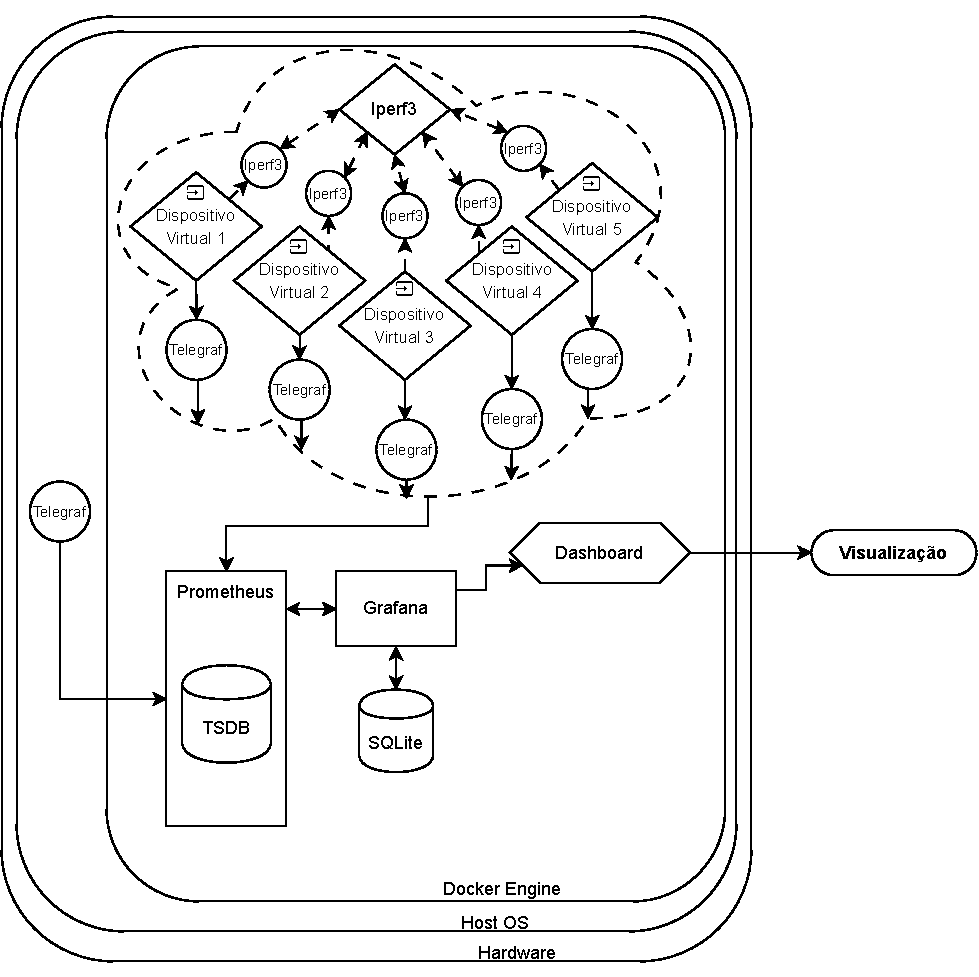
\includegraphics[width=\textwidth]{Imagens/chap04/by-blocks/dashboard_diagram.pdf}
\caption{Visualização.}
\label{fig:DiagramaVisualizacao}
\end{figure}


}

{\color{blue}
\section{Dashboards}

\begin{enumerate}  
  \item comentar sobre sobre as coisas que o provisioning já adiantou (datasource padrão, por exemplo);
  \item a normalização dos dados usando o Pormetheus Recording Rules
  \item Criação dos filtros globais (Grafana Variables);
  \item Regras globais (span e refresh rate);
  \item Falar de cada gráfico, justificando visualizações, comentando sobre as queries/cálculos e colocar imagens;
  \item Quando chegar em CPU, explicar o porquê de haver picos acima de 100\% mesmo com a limitação de cpu (olhar pasta docs/cpu\_shares)
  \item Quando chegar na seção de disco, apresentar o estudo de caĺculo do df (motivação e resultados);
  \item Chegando na parte de redes, justificar o porquê de nao termos dados de drop e erro de pacotes (apresentar o estudo de caso de camadas de rede e aplicação);
  \item Fechamento explicando a exportação do JSON e seu versionamento e carregamento automatico via docker volume;
\end{enumerate}


\section{Alarmes e Notificações}
\label{section:AlarmesNotificacoes
}
\begin{enumerate}
  \item Comentar sobre o Alertmanager e a sua configuração;
  \item Explicar como adicionei o servidor smtp do gmail e as tentativas falhas com o Telegram;
  \item Configuração das regras de notificação e os pontos de contato;
  \item Como utilizei, a primeiro momenot, a UI do Grafana para criar os alertas (isso era interessante pq vinculava automaticamente o alerta ao respectivo gráfico);
  \item Como, assim como no dashboard, eu exportava e versionava tudo via JSON;
  \item Problemas do SQLite e a migração para o Postgres (explicitar como a migração foi fácil graças ao provisionamento, versionamento, uso do Docker e TSDB fazendo o trabalho de persistência);
  \item Migração para o Alertmanager+TSDB (enfatizar como tudo fica embutido no Prometheus e como isso simplifica a arquitetura);
  \item EDITAR DIAGRAMAS (SQLite vira POSTGRES)
\end{enumerate}


}


\section{Caso de Uso}
\label{section:CasosDeUso}

O caso de uso seria o monitoramento ( exemplo: eu estou monitorando a minha maquina com o meu projeto)

% \textcolor{blue}{Dúvida: Como combinamos de contar a experiencia com o SQLitexPostgres e tambem a alteração para Alertmanager na seção 3.5 (alertas e dashboards), confesso que não sei mais o que colocar aqui... talvez matemos essa subseção 3.2.6?}

% Uma dúvida que tive hoje nesta seção: nós combinamos de comentar sobre dashboards e alertas na seção 3.5, porém isso implica que eu não incluiria os respectivos blocos de dashboards e alertas (e Alertmanager) no diagrama neste momento. Isso implica que a figura do diagrama final da arquitetura só apareceria no fim da seção 3.6. Como proceder?

% Aqui a finalizo a seção contando a historia do SQLite x Postgres e eventualmente chegando na decisão de descartar ambos e ficar apenas com o TSDB.
% Tambem relato da minha experiencia de formatar a maquina toda e a facilidade em subir todo o projeto (salve a configuração pontual do permissionamento de escrita do grafana e da chave do repositorio do telegraf)
% Após isso eu fecho a seção com o diagrama da arquitetura final definitiva. 


% foram feitas tentativas de utilização de ferramentas de \foreign{chaos-engineering} como Pumba e ChaosBlade e até mesmo tentativas de manipulação direta de iptables para gerar tráfego de rede, mas essas ferramentas não se mostraram adequadas para este trabalho.


% Por debaixo dos panos, ferramentas de \foreign{chaos testing} utilizam para testes de rede o módulo \verb|netem| do sistema de controle de tráfego \verb|tc| do Linux. Esse sistema opera na camada de controle de tráfego (\verb|qdisc|). Enquanto isso, o \foreign{plugin} \verb|inputs.net| do Telegraf a partir da leitura do \verb|procfs/net/dev|, que se encontra na camada de interface de rede. Ou seja, 


\begin{figure}[H]
\centering
\setlength{\abovecaptionskip}{-20pt}
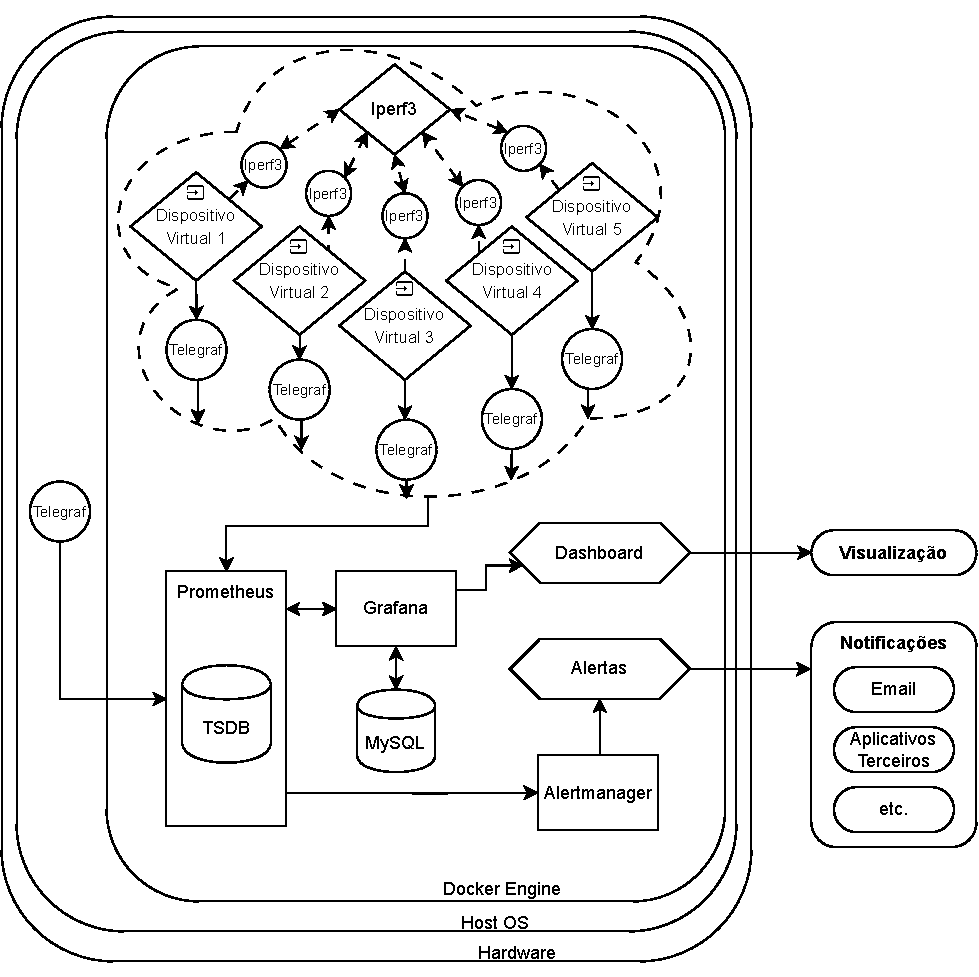
\includegraphics[width=\textwidth]{Imagens/chap04/by-blocks/alerts_diagram.pdf}
\caption{Notificações e Arquitetura Final.}
\label{fig:DiagramaAlertas}
\end{figure}


\begin{figure}[H]
\centering
\setlength{\abovecaptionskip}{-20pt}
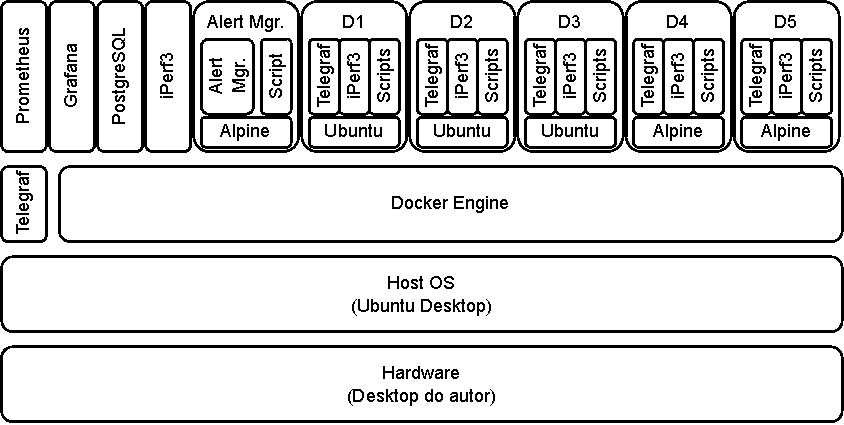
\includegraphics[width=\textwidth]{Imagens/chap04/final_stack.pdf}
\caption{\foreign{Stack} final.}
\label{fig:StackFinal}
\end{figure}

